\documentclass[12pt]{article}
\usepackage{sbc-template}
\usepackage{graphicx}
\usepackage{amsmath}
\usepackage{subfigure}
\usepackage{times,amsmath,epsfig}
\usepackage{graphicx,url}
  \makeatletter
  \newif\if@restonecol
  \makeatother
  \let\algorithm\relax
  \let\endalgorithm\relax
\usepackage[lined,algonl,ruled]{algorithm2e}
\usepackage{multirow}
\usepackage[brazil]{babel}
\usepackage[utf8]{inputenc}
\usepackage[pdftex]{hyperref}

\sloppy

\title{Algoritmos e Estruturas de Dados 3 \\ Trabalho Prático 6 \\
\huge{Auxiliar de Redação}}
\date{November 22, 1963}


\author{André Taiar Marinho Oliveira}


\address{Departamento de Ciência da Computação -- Universidade Federal de Minas Gerais (UFMG)
\email{taiar@dcc.ufmg.br}
\\
\\ Dezembro de 2010
}

\begin{document}

\maketitle

\begin{resumo}
\label{resumo}
Este relatório descreve a implementação de um sistema de auxílio à confecção de textos que, baseado em algumas premissas sobre más práticas para redação e estatísticas sobre palavras, frases, parágrafos e linhas, consegue indicar alguns pontos em que o texto pode ser melhorado. Foram sugeridas 3 situações em que o programa poderia indicar uma melhora das quais 2 foram implementadas. A primeira trabalha com estatísticas sobre os textos, indicando a ocorrência de parágrafos formados por apenas uma sentença, sentenças muito longas ou muito curtas (as análises também são feitas considerando e ignorando \textit{stop words} \footnote{Stop Words são palavras consideradas sem valor semântico para a análise de tópico de um texto (como artigos e preposições, por exemplo). \href{http://searchenginewatch.com/2156061}{Referência}.} ). A última trabalha com algumas expressões que são frequentemente utilizadas em uma língua mas teóricamente não existem e por isso devem ser evitadas nos textos.
\end{resumo}

\section{Introdução}
\label{introducao}

Uma cadeia de caracteres é uma sequência qualquer de elementos que podem ser representados como caracteres. Elas aparecem em várias áreas da computação: processamento de textos em linguagem natural, códigos, dicionários, sequenciamento de DNA em biologia computacional, representação de imagens por meio de bitmaps, entre outros. Neste trabalho, utilizamos a representação de um texto em linguagem natural como uma cadeia de caracteres e utilizamos algoritmos de processamento de cadeias de caracteres para reconhecer diversas informações pertinentes às análises que desejamos fazer.

Neste cenário, 2 tipos de algoritmos foram utilizados, um para cada situação a ser analisada. O primeiro foi um algoritmo baseado em autômato. Foi melhor abordar a modelagem dessa etapa com um autômato finito por se tratar de um parsing da cadeia de caracteres aonde diversos estados podem ser definidos, facilitando a análise com uma máquina de estados. O outro algoritmo, utilizado para resolver a etapa 3, foi um algoritmo de força bruta (que é o algoritmo mais simples para casamenfaz a leitura inicial do arquivo de entrada e trabalha com os módulos Camadas e Simulação. Faz a contagem do tempo de execução das partes principais do programa para análise de complexidadeto de cadeias de caracteres). Mais detalhes sobre os algoritmos serão vistos na sessão \ref{solucao_proposta}.

Tanto as \textit{stop words} quanto as expressões e duas entradas de teste foram préviamente fornecidas pelos monitores para que pudéssemos rodar e testar o trabalho. Foi uma condição assumida que o texto não teria qualquer tipo de acentuação, portanto os arquivos de entrada, \textit{stop words} e expressões foram tratados e organizados para isso.

\section{Solução Proposta}
\label{solucao_proposta}

\subsection{Etapa 1}
\label{etpu}
Na Etapa 1 o programa deveria fornecer para cada parágrafo do texto:
\begin{enumerate}
  \item O número da linha no arquivo fonte aonde o parégrafo começa;
  \item o número de sentenças no parágrafo;
  \item para cada sentença, o número de palavras dela incluindo e não incluindo \textit{stop words}.	
\end{enumerate}

Respeitando as considerações feitas feitas na especificação acerca de marcação de parágrafos e palavras e sobre pontuação, foi elaborado um autômato que reconhece esse tipo de marcação no texto lendo a cadeia de caracteres um a um. Um exemplo do autômato pode ser visto na figura \ref{img:automato}.

\begin{figure}[ht!]
\centering
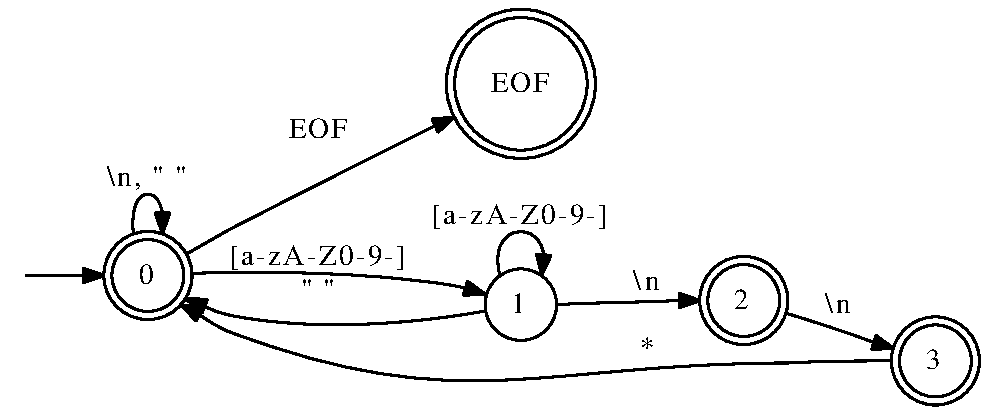
\includegraphics[width=10.0cm]{automato.pdf}
\label{img:automato}
\caption{Autômato de reconhecimento do texto}
\end{figure}

Em cada estado final ele retorna um sinal para que saibamos o que fazer com o valor capturado.
\begin{itemize}
  \item $1 \longrightarrow 0$ - casou uma palavra;
  \item $1 \longrightarrow 2$ - casou uma palavra;
  \item $2 \longrightarrow 3$ - casou um parágrafo;
  \item $3 \longrightarrow 0$ - é uma transição vazia ($\lambda$);
  \item $0 \longrightarrow EOF$ - retorna o fim do arquivo.
\end{itemize}

Dessa forma conseguimos interpretar o que está acontecendo com o texto à cada caractere que lemos da nossa cadeia, contabilizando semânticamente o que precisamos. As \textit{stop words} que devemos desconsiderar estão em um arquivo que é carregado na memória antes de varrermos o texto seguindo o autômato. Com as palavras em memória, vamos contabilizando as palavras que são e que não são \textit{stop words} à medida que o autômato casa os padrões. 

Como as \textit{stop words} estão ordenadas no arquivo que é passado, conseguimos determinar se uma palavra é ou não é relevante com uma ordem de complexidade menor do que $O(n)$. Assim, a complexidade total do algoritmo é $O(n)$; onde $n$ é o número de caracteres na cadeia de entrada (o número de caracteres do texto). Processando o texto como um autômato, precisamos apenas de uma passada para obter as informações que desejamos.

\subsection{Etapa 2}
Por ser opcional e pela falta de tempo de implementar a Etapa 2 do trabalho não foi implementada e não será discutida nem analisada no trabalho.

\subsection{Etapa 3}
\label{etpt}
Na Etapa 3 temos uma lista de expressões que não existem na língua portuguesa mas que costumam aparecer em alguns textos. Por isso, devemos localizá-las e indicar a linha em que ocorrem no texto. O algoritmo funciona carregando primeiramente a lista das expressões em memória. Em seguida, para cada uma das expressões, varremos o texto uma vez tentando casar a expressão com uma algoritmo de força bruta. Segue o pseudo-código do algoritmo:

\begin{algorithm}[h!]
\begin{footnotesize}
String $texto \longleftarrow$ cadeia de caracteres que vamos explorar\;
String $padrao\longleftarrow$ padrão que deve ser encontrado na cadeia de caracteres\;

\For{int $i=0$; $i < (length(texto) - length(padrao) + 1)$; $i+=1$}
{
  int $k = 1$\;
  int $j = 0$\;
  \While{$(j < m)$ \& $texto[k] == padrao[j]$}
  {
  	$j += 1;$
  	$k += 1;$
  	\If{$j == m$}
  	{
  		\Return "casou"\;
  	}
  }
}

\caption{Algoritmo de casamento de padrões por força bruta}
\end{footnotesize}
\end{algorithm}

Este algoritmo tem ordem $O(m * n)$ sendo $m$ o tamanho da cadeia de caracteres do texto e $n$ o tamanho da cadeia de caracteres do padrão a ser encontrado. Como fazemos isso para cada expressão em nossa lista de expressões, a complexidade total do algoritmo é $O(m * n * o)$; sendo $o$ o número de expressões que devemos checar.

\section{Código}

\subsection{Módulos}
O programa foi separado em seis módulos:
\begin{itemize}
\item \textbf{Entrada e Saída:} define os campos necessários para ler as informações da linha de comando e dos arquivos e trabalha com os arquivos de entrada e saída. Também contém uma função muito importante que segue o autômato descrito na figura \ref{img:automato} lendo um \textit{token} \footnote{Token em computação é um segmento de texto ou símbolo que pode ser manipulado por um parser, que fornece um significado ao texto; em outras palavras, é um conjunto de caracteres (de um alfabeto, por exemplo) com um significado coletivo.} do arquivo de entrada.
\item \textbf{Etapa 1:} implementa o algoritmo descrito em \ref{etpu}.
\item \textbf{Stop Words:} é utilizado pelo módulo \textbf{Etapa 1} para discenir as palavras úteis das \textit{stop words}. Carrega uma lista de palavras de dentro de um arquivo para a memória e libera a memória também. Busca uma palavra para ver se ela é ou não uma \textit{stop word}.
\item \textbf{Etapa 3:}  implementa o algoritmo descrito em \ref{etpt}.
\item \textbf{Expressões:} carrega a lista de expressões que deve ser reconhecida pela módulo \textbf{Etapa 3} em memória e libera a memória também.
\item \textbf{Principal:} interage com todos os outros módulos fazendo com que as estruturas sejam carregadas em memória e descarregadas em seguida. Contabiliza os tempos de execução do programa para análise de complexidade.
\end{itemize}

\subsection{Entrada e saída}
\subsubsection{Linha de comando}
\label{linha_de_comando}
Para não haver problemas com a leitura da linha de comando, foi utilizado um utilitário do
sistema Linux chamado \textbf{getopt} que permite uma leitura mais robusta dos argumentos
passados ao programa. O comando para execução do programa definido para a linha de entrada 
foi:
\begin{verbatim}
#: ./tp6 -i <I> -o <O>
\end{verbatim}
Sendo: 
\begin{itemize}
  \item \textbf{I} - Arquivo de entrada;
  \item \textbf{O} - Prefixo utilizado nos nomes dos arquivos de saída.
\end{itemize}

\subsubsection{Formato da entrada}
Não existe um formato padronizado para os arquivos de entrada. Inicialmente foram passados arquivos em português, \textit{stop words} em português e expressões indevidas em português, todos sem acentuação. O sistema funcionaria para qualquer língua com as mesmas considerações feitas nas etapas 1, 2 e 3 desde que o arquivo de \textit{stop words} e o de expressões fosse na mesma língua.

O arquivo de \textit{stop words} chama-se stopwords.txt e está junto com os arquivos do programa juntamente com o expressoes.txt.

\subsubsection{Formato da saída}
O programa tem uma saída para cada etapa diferente. O nome do arquivo de saída da etapa $i$ tem o formato $sufixo_{i}$; onde o $sufixo$ é o parâmetro passado na linha de comando como descrito em \ref{linha_de_comando}.

\begin{itemize}
  \item \textbf{Etapa 1}: 
  \begin{verbatim}
Parágrafo 1 começa na linha 1
Frase 1
Com stop words: X1
Sem stop words: Y1
Frase 2
Com stop words: X2
Sem stop words: Y2
...
Frase N
Com stop words: XN
Sem stop words: YN
...

Parágrafo P começa na linha L
Frase 1
Com stop words: X1
Sem stop words: Y1
Frase 2
Com stop words: X2
Sem stop words: Y2
...
  \end{verbatim}
  \item \textbf{Etapa 3}: 
  \begin{verbatim}
Expressao: "expressao 1"
Linha: a
...
Linha: b
Expressao: "expressao 2"
Linha: l
...
Linha: m
...
Expressao: "expressao n"
Linha: p
...
Linha: q
  \end{verbatim}
\end{itemize}

\subsection{Compilação}
O compilador utilizado neste trabalho foi o GCC (adotado como padrão para a disciplina) e 
o comando para compilar o programa através do GCC é:\\
\\
\#: gcc -o tp6 tp6.c expressoes.c expressoes.h stopWords.c stopWords.h etapa1.c etapa1.h etapa3.c etapa3.h io.c io.h\\
\\
caso estejam todos os arquivos dentro do mesmo diretório.

Como pedido na especificação, foi feito um arquivo Makefile com o qual é possível compilar
o programa com o comando: 
\begin{verbatim}
  #: make main
\end{verbatim}

E podemos compilar e executar o programa com o comando:
\begin{verbatim}
  #: make run
\end{verbatim}
que fará, além da compilação, com que o programa execute com uma entrada pequena.

\section{Avaliação Experimental}
\label{avaliacao_experimental}
Assim como utilizado no livro \textit{Projeto de Algoritmos com implementaçes em Java e C++}, para criar textos com ordens de grandeza de diferença foi construído um script que gera textos aleatórios. Variamos nestes textos o número de palavras de cada um. Fizemos várias execuções variando o tamanho do texto de entrada e obtivemos tempos mostrados na tabela e no gráfico abaixo:



\section{Conclusões}
\label{conclusao}
Neste trabalho foi desenvolvido um sistema simples que ajuda no processo de redação de textos em português. Este sistema tem 2 funções principais:
\begin{itemize}
  \item De acordo com a \textbf{Etapa 1} do trabalho, o sistema mostra o tamanho das frases nos parágrafos e quantas frases utilizamos dentro de um mesmo parágrafo. Assim, podemos ser cautelosos e evitar parágrafos formados por uma única sentença, sentenças muito longas ou sentenças muito curtas, ou mesmo uma mistura dessas situações.
  \item De acordo com a \textbf{Etapa 3} do trabalho, o sistema mostra o uso de algumas expressões que, apesar de utilizadas na prática, não existem na língua portuguesa. Apontando em quais linhas do texto tal expressão ocorre, ele nos auxilia a evitar tais construções.
\end{itemize}

Na \textbf{Etapa 1}, o algoritmo utilizado baseado em um autômato finito, nos possibilitou processar o texto de forma eficiente. Na  \textbf{Etapa 3}, o algoritmo de força bruta pode adquirir uma complexidade $O(n^{3})$ dependendo do número de expressões que vamos buscar no texto e do tamanho da cadeia de caracteres de cada expressão. Na prática este número é bem melhor (como visto no livro \textit{Projeto de Algoritmos com implementaçes em Java e C++}, pg. 325 \textbf{Algoritmo Força Bruta}).

\end{document}
